\documentclass{scu-thesis}
\usepackage{amsmath}	% for advanced typesetting of mathematics
\usepackage{graphicx}	% for including graphics
\usepackage{natbib}	% for better citation styles
\usepackage{txfonts}	% for using the Times-Roman font


% These must be set first ... the rest of the thesis commands rely on them.

\author{Manoj Adhikari}
\author{Colby Harper}
\author{Sean Karstein}
\title{On the Construction of Matter, or Is There a God Particle?}
\department{Department of Computer Engineering}
\degree{Bachelor of Science in Computer Science and Engineering}


% Only bachelor's theses should have multiple authors and/or be from
% multiple departments.  Signatures required:
%
% Bachelor's theses: advisor(s), department chair(s)
% Master's theses: advisor, reader, department chair
% Doctoral theses: doctoral committee (including advisor), department chair

\begin{document}
\frontmatter
\signature{Thesis Advisor}
\signature{Thesis Advisor}
\signature{Department Chair}
\signature{Department Chair}

\maketitle
\begin{abstract}
Taking group photos during important events is a common practice. Group photos are taken to remember cheerful times when people had opportunity to meet many other people. However, an unappealing facial experience of one person can easily ruin the entire photo. Capturing the wrong moments when a person doesn't look attractive can leave him/her displeased from the complete event experience. A solution is to develop a mobile app that captures the moment when everyone is smiling with eyes wide open. Our solution aims to develop an iPhone app that will preclude users from worrying about not having a great group picture. 
\end{abstract}


\tableofcontents
\listoffigures

\mainmatter
\chapter{Introduction}
Taking pictures to save our best memories is a common practice. During group pictures, photos can be entirely ruined by a single person?s expressions. We all have seen photos of people who did not smile/looked away, or worse, been that person. The experiences at big events and gatherings would be much more fulfilling if we didn?t have to take many pictures just to get a nice smiling photo. Modern cameras and phones have beautiful design incorporated with advanced features. However, they have forgotten to address this pesky issue that would uplift everyone?s picture taking moment. 

Currently, the only group photo technology to be created is the automatic photo with timer.  The purpose of this is to eliminate the need for someone to click the button to take the photo, however it is not smart.  It does not signal when the photo will be taken, and takes the photo only when the timer has reached zero.  Therefore, this does not have any effect on the quality of the photo.  Currently, the only solutions affecting the quality of group photos are after effect softwares such as photoshop.  However, these often require a large amount of money, and a level of skill in using the product, which most people don?t have.

We propose to build an iOS app that utilizes the iPhone?s camera and adds the feature of taking pictures automatically when everyone in the group is looking at the camera with their eyes open and smiling. The app will automate the tedious task of capturing the right moment saving people?s time for actually enjoying the moment.  Computer vision will be used to narrow the focus of the image, to then allow a machine learning model to determine when the right moment to snap the photo is.

To conclude, our design will accomplish two things: firstly, it will save time for both people who are getting their photo taken as well as the person taking the photo, as the camera will know exactly when to take the right photo, and secondly, will improve the quality of photos, allowing for memories to be better cherished by all. 




\chapter{Requirements}

\section{Functional Requirements}
Critical:
\begin{itemize}
 \item Users can take pictures using iPhone camera.
 \item Users can choose to save or disregard the photo captured.
 \item The app can identify if everyone in the group is smiling with eyes wide open or not.
 \item Photos are automatically captured without users click.
 \end{itemize}
 
Recommended:
\begin{itemize}
\item Users can share pictures with their friends using phone numbers.
 \end{itemize}
 
Suggested:
\begin{itemize}
\item Users can give feedback on whether the app captured good pictures.
\item The system will offer photo editing features
 \end{itemize}
 
\section{Non-Functional Requirements}
Critical: 
\begin{itemize}
\item The user interface will be simple and intuitive 
\item The system will be easy to install and use.
 \end{itemize}
 
Recommended:
\begin{itemize}
\item The system will be secure from unauthorized users. 
 \end{itemize}
 
Suggested:
\begin{itemize}
\item The system will be high performance and will require minimal system resources.
 \end{itemize}
\section{Design Constraint}
\begin{itemize}
\item The app can only run on iPhones with iOS versions starting iOS  10.3.
 \end{itemize}


\chapter{Use Cases}
Use case diagrams demonstrate how users will interact with our system. In our case, users will be able to take photos, then accept or reject them.

\begin{figure}[!h]
    \centering
    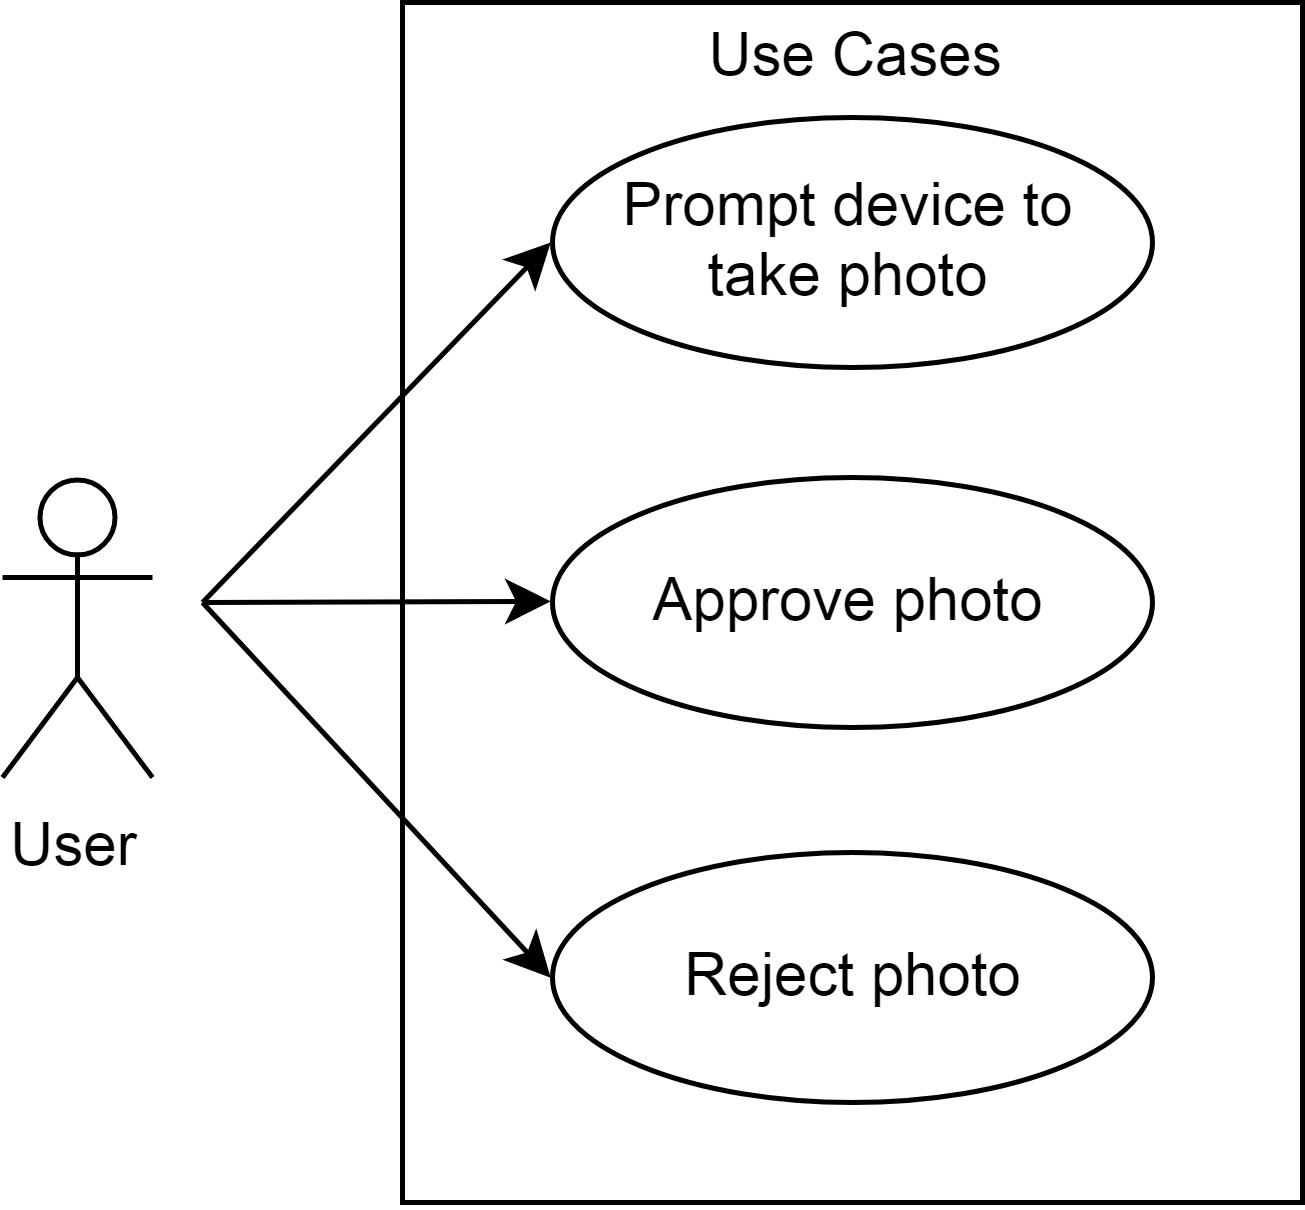
\includegraphics[scale=0.25]{usecasediagram}
    \caption{Figure 3.1: Use Cases}
    \label{fig:usecasediagram}
\end{figure}

\begin{enumerate}
    \item Prompt device to take photo
    \begin{enumerate}
        \item Goal: Take photo
        \item Actors: User
        \item Pre-conditions: 
            \begin{enumerate}
                \item Application must be open on device
            \end{enumerate}
        \item Steps:
            \begin{enumerate}
                \item User presses button to prompt device to take photo
            \end{enumerate}
        \item Post-conditions:
            \begin{enumerate}
                \item None
            \end{enumerate}
        \item Exceptions:
            \begin{enumerate}
                \item Application must have device permission to use camera
            \end{enumerate}
    \end{enumerate}
\end{enumerate}

\begin{enumerate}
    \item Approve photo
    \begin{enumerate}
        \item Goal: Save photo to phone storage
        \item Actors: User
        \item Pre-conditions: 
            \begin{enumerate}
                \item Must have taken a photo
            \end{enumerate}
        \item Steps:
            \begin{enumerate}
                \item User presses accept button when prompted after taking a photo
            \end{enumerate}
        \item Post-conditions:
            \begin{enumerate}
                \item None
            \end{enumerate}
        \item Exceptions:
            \begin{enumerate}
                \item None
            \end{enumerate}
    \end{enumerate}
\end{enumerate}

\begin{enumerate}
    \item Reject photo
    \begin{enumerate}
        \item Goal: Delete photo and try again
        \item Actors: User
        \item Pre-conditions: 
            \begin{enumerate}
                \item Must have taken a photo
            \end{enumerate}
        \item Steps:
            \begin{enumerate}
                \item User presses reject button when prompted after taking a photo
            \end{enumerate}
        \item Post-conditions:
            \begin{enumerate}
                \item None
            \end{enumerate}
        \item Exceptions:
            \begin{enumerate}
                \item None
            \end{enumerate}
    \end{enumerate}
\end{enumerate}


\chapter{Activity Diagram}

The flowchart outlines the workflow of all users actions and interactions with the system. The diagram does not show system actions, such as processing the image stream and deciding when to capture an image.

\begin{figure}[!h]
    \centering
    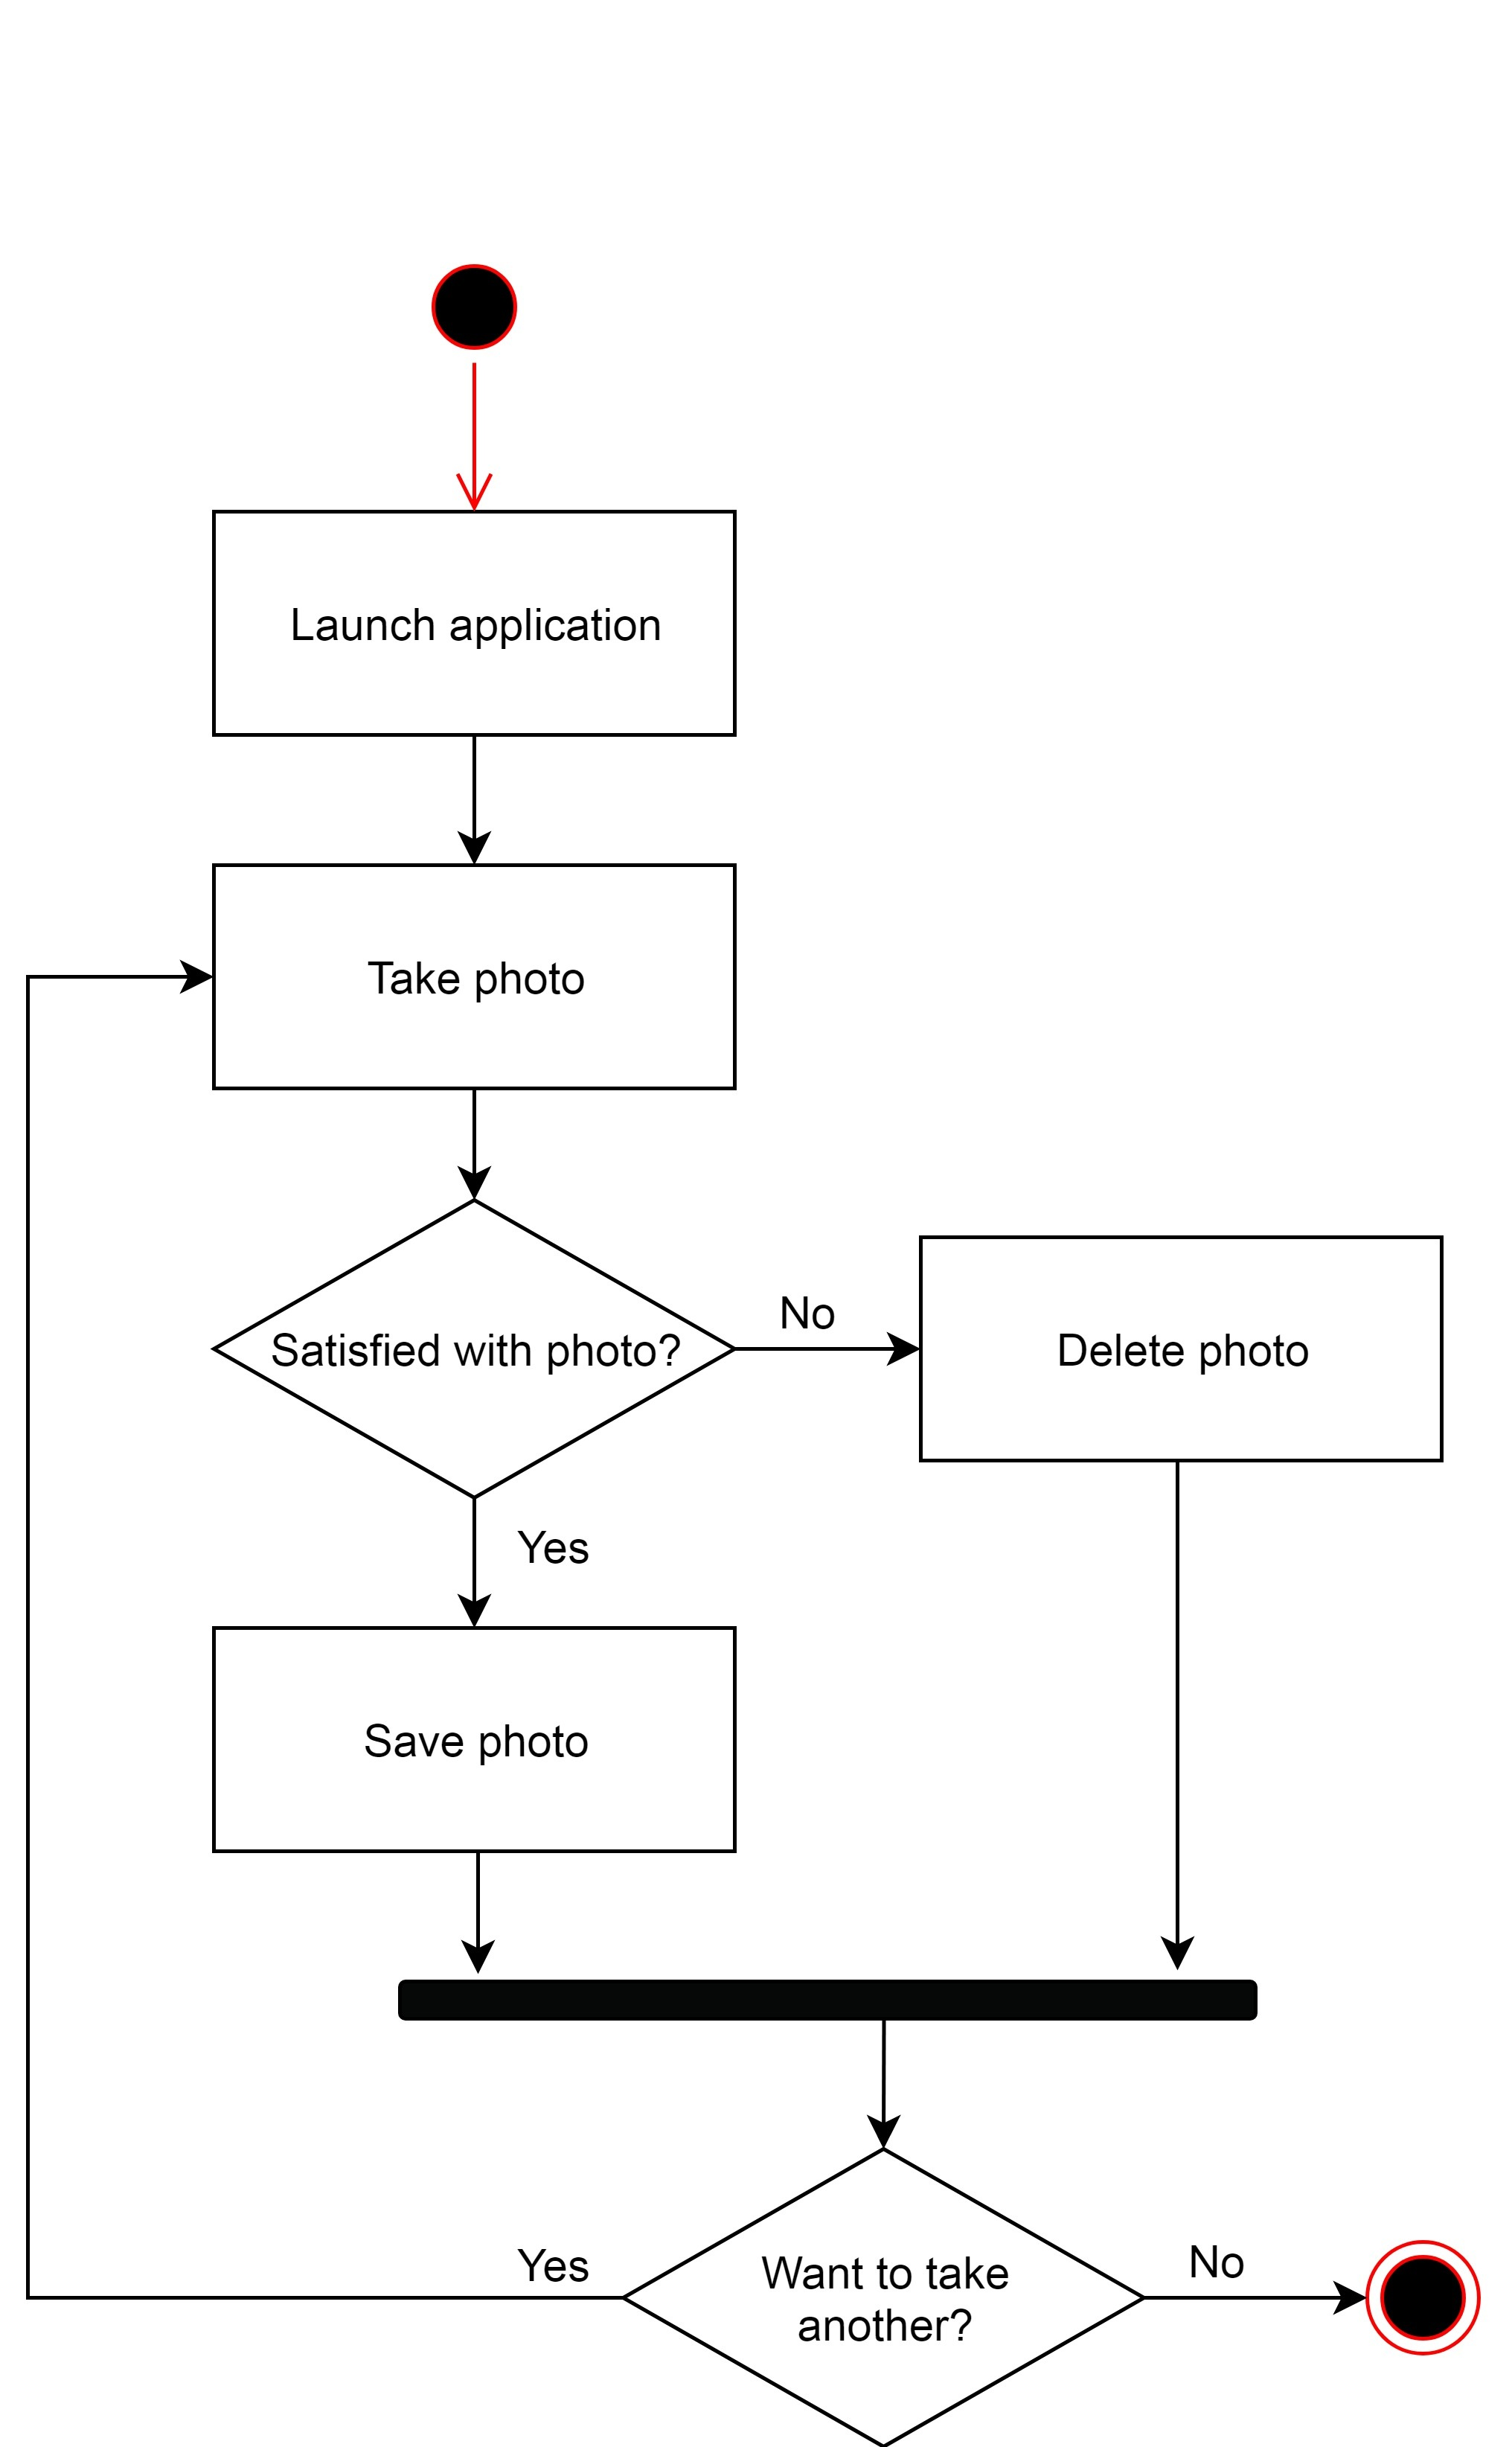
\includegraphics[width=0.75\textwidth]{activitydiagram}
    \caption{Figure 4.1: Work flow of user interacting with system}
    \label{fig:activitydiagram}
\end{figure}

\chapter{Conceptual Model}

Users will navigate to the application on an iPhone to begin using the system. Upon launching the app, a camera feed appears, as shown in Figure 5.1. They can press the camera icon to prompt the device to take a photo. 

\begin{figure}[!h]
    \centering
    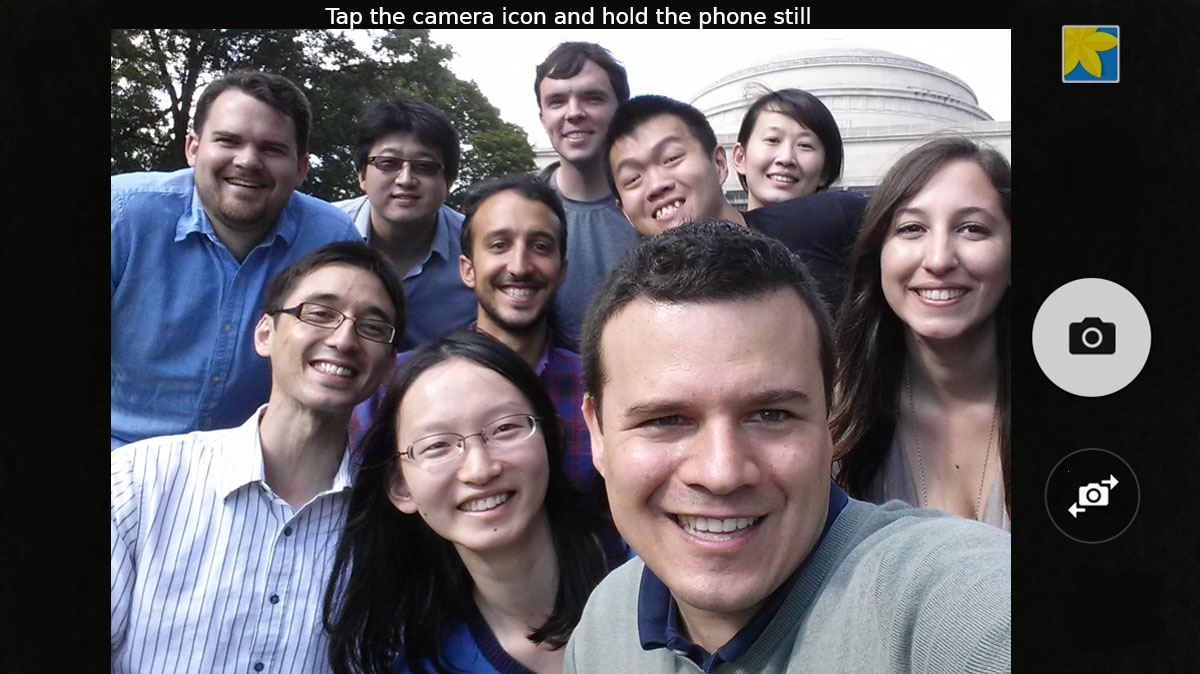
\includegraphics[width=0.75\textwidth]{conceptualmodel1}
    \caption{Figure 5.1: Mockup of camera user interface}
    \label{fig:conceptualmodel1}
\end{figure}

After they has pressed the camera button, the application will wait until all subjects are in frame with their eyes open to capture the image. Upon capturing the image, they will be greeted with an alert asking whether they want to save the photo or reject it, as seen in Figure 5.2.

\begin{figure}[!h]
    \centering
    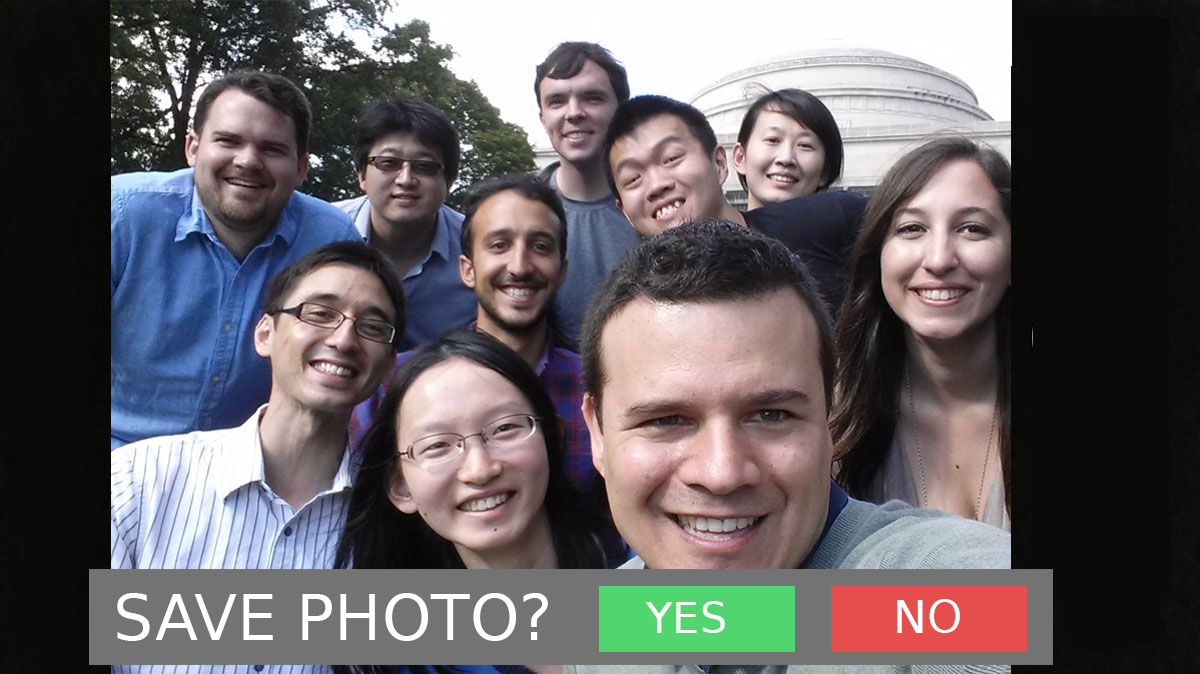
\includegraphics[width=0.75\textwidth]{conceptualmodel2}
    \caption{Figure 5.1: Mockup demonstrating the approval dialogue}
    \label{fig:conceptualmodel2}
\end{figure}

If the user chooses to accept the photo, then it will be saved to the user's storage and they will return to the camera screen. If the user chooses to discard the photo, then it will be delete and they will return to the camera.


\chapter{Architectural Diagram}

We plan to utilize a data flow architecture to complete this project as shown in Figure 6.1.

\begin{figure}[!h]
    \centering
    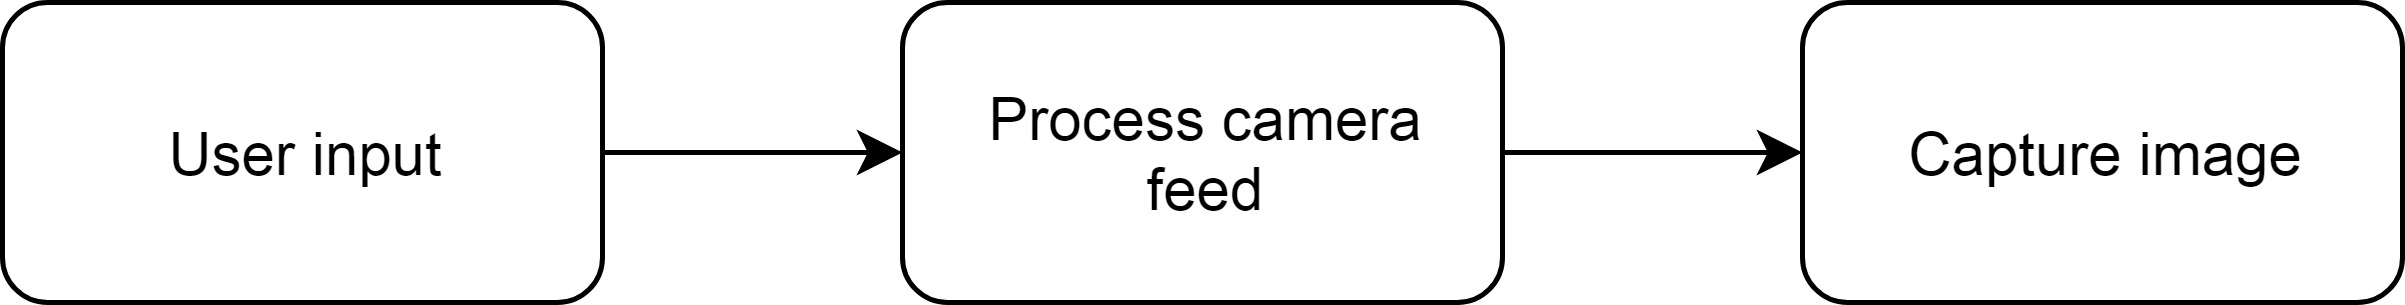
\includegraphics[width=0.75\textwidth]{architecturediagram}
    \caption{Figure 5.1: Data Flow Architecture}
    \label{fig:architecturediagram}
\end{figure}

Users will provide input with their phone's touchscreen, which triggers the device to begin analyzing the camera feed. Once the system determines the input is acceptable, it captures the image. 



\chapter{Activity Diagram}

The flowchart outlines the workflow of all users actions and interactions with the system. The diagram does not show system actions, such as processing the image stream and deciding when to capture an image.

\begin{figure}[!h]
    \centering
    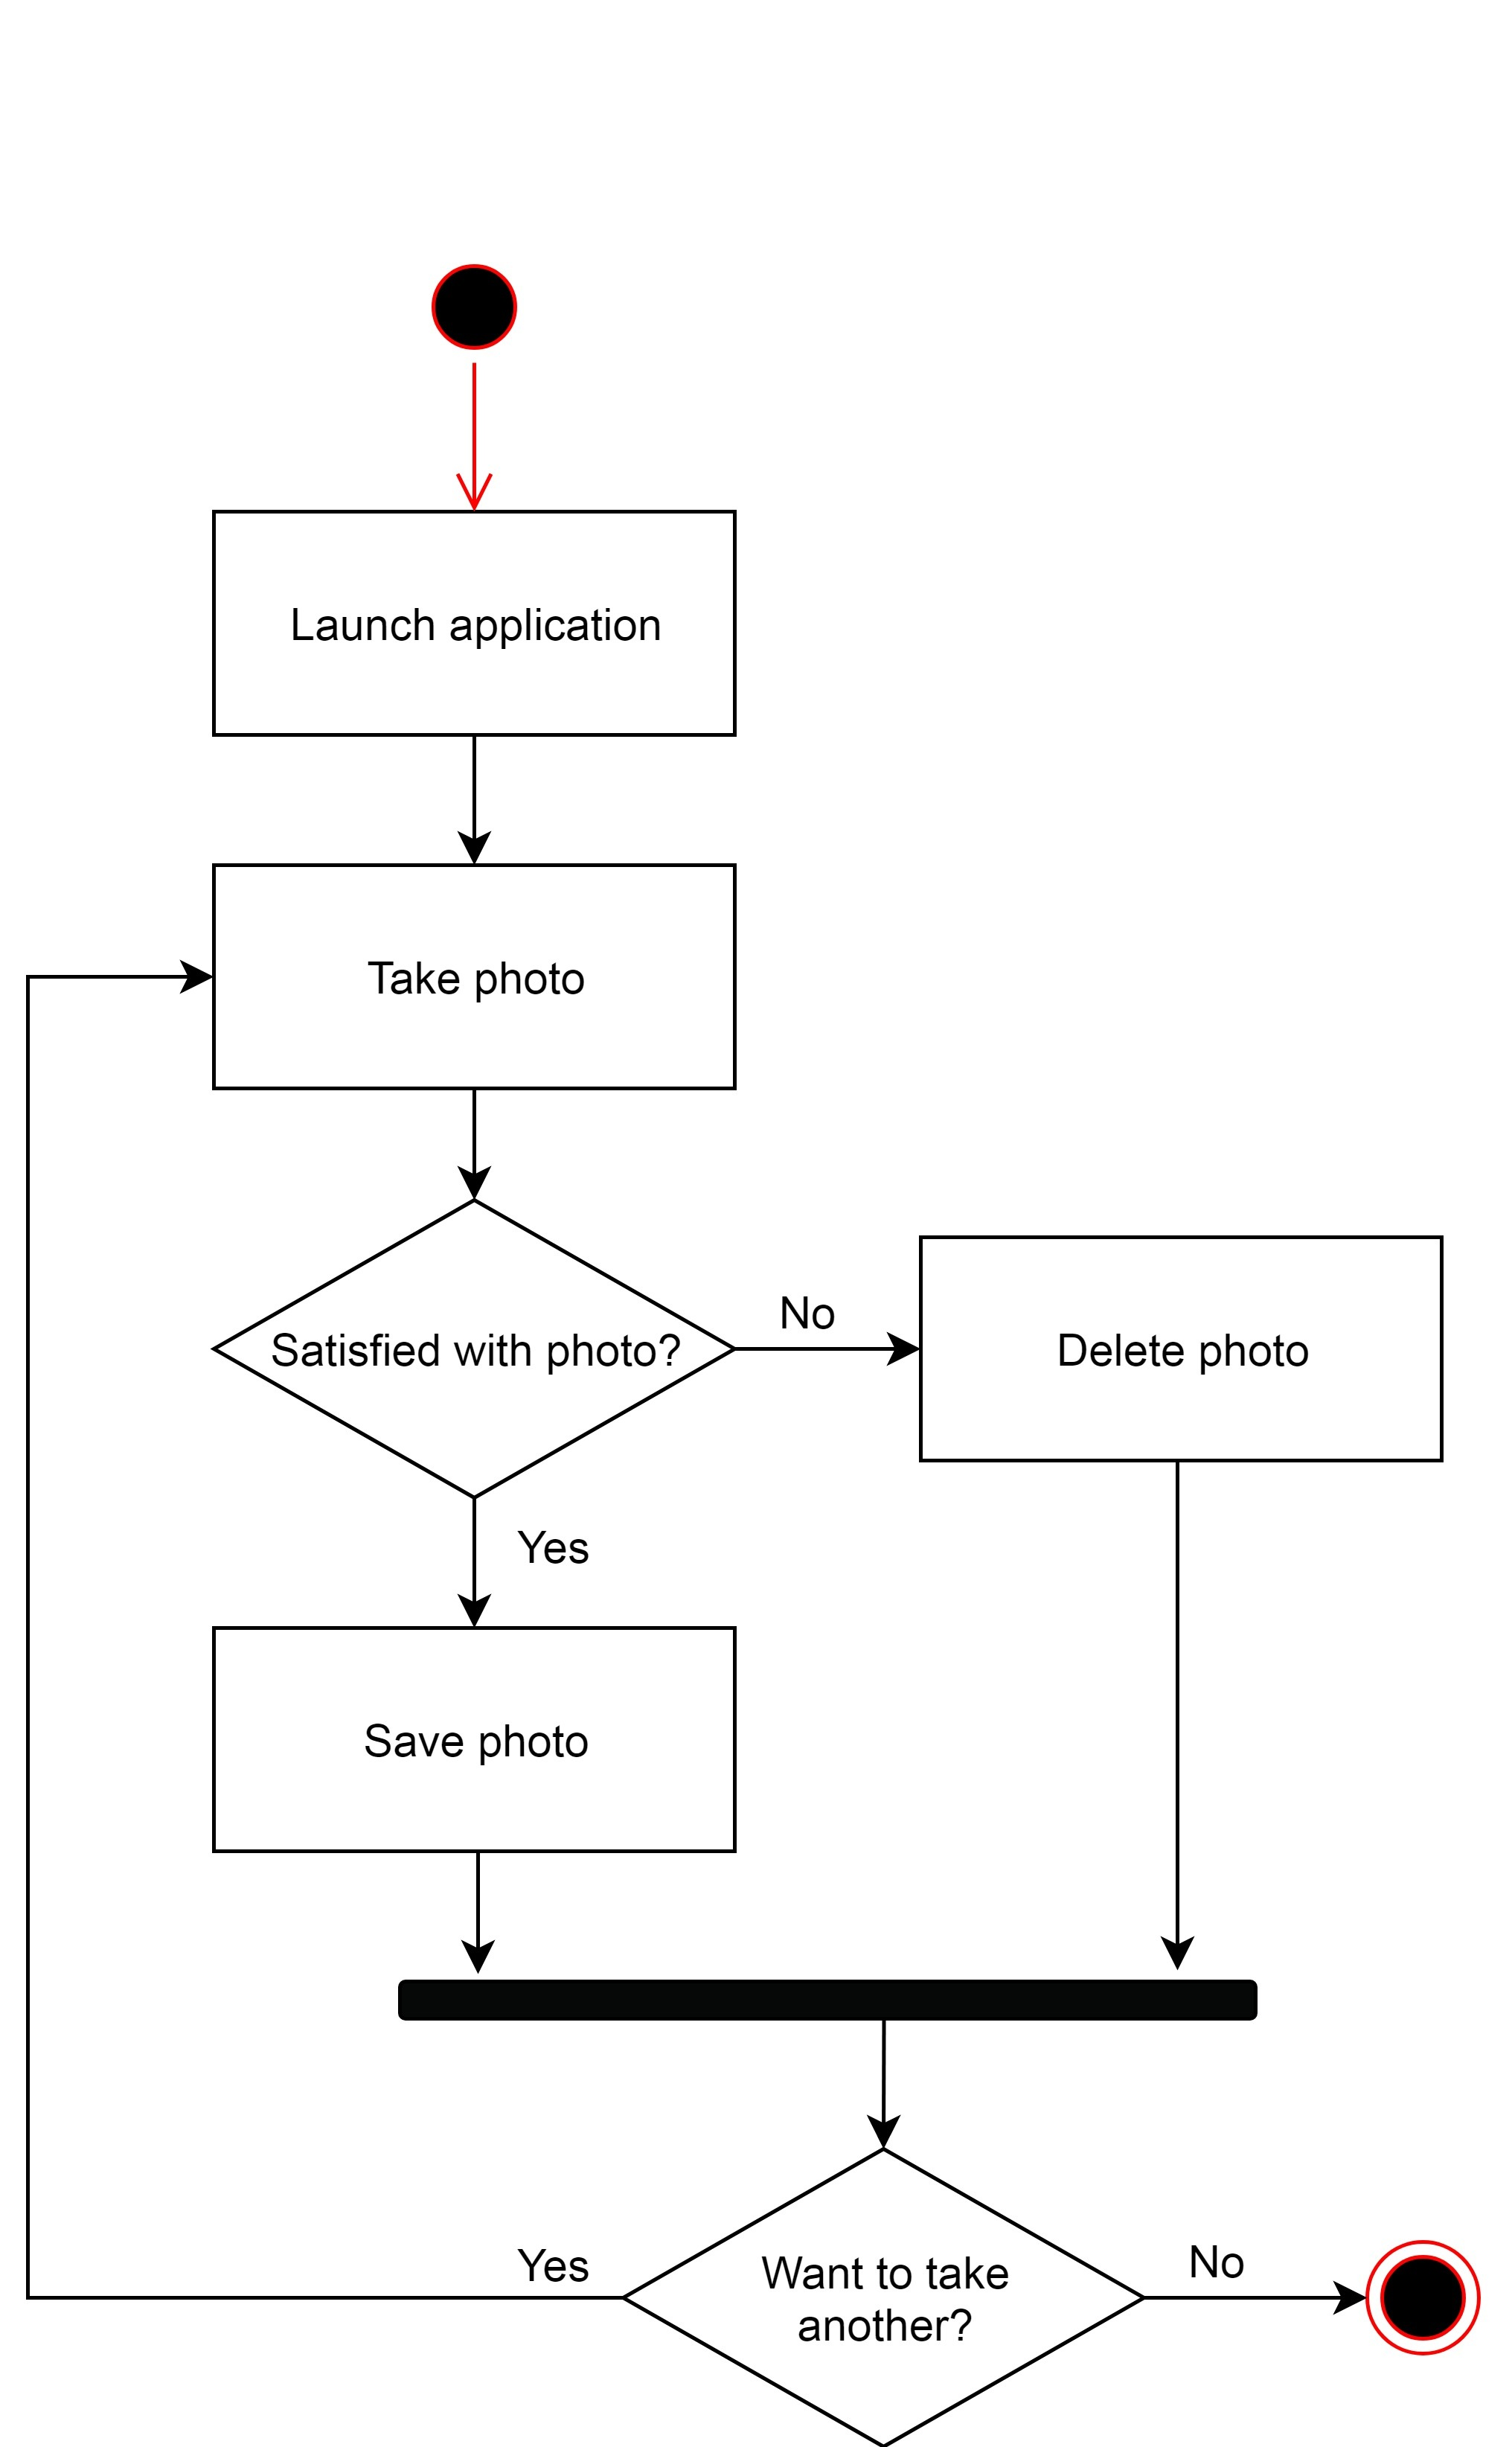
\includegraphics[width=0.75\textwidth]{activitydiagram}
    \caption{Figure 4.1: Work flow of user interacting with system}
    \label{fig:activitydiagram}
\end{figure}




\chapter{Conceptual Model}

Users will navigate to the application on an iPhone to begin using the system. Upon launching the app, a camera feed appears, as shown in Figure 5.1. They can press the camera icon to prompt the device to take a photo.

\begin{figure}[!h]
    \centering
    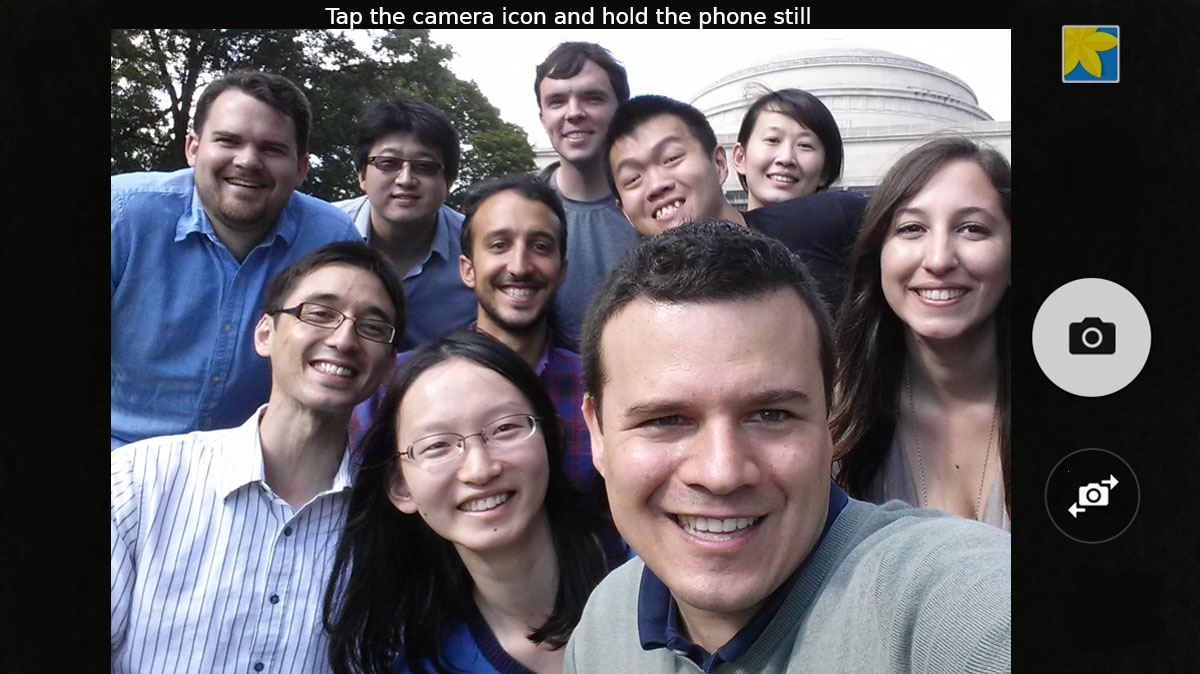
\includegraphics[width=0.75\textwidth]{conceptualmodel1}
    \caption{Mockup of camera user interface}
    \label{fig:conceptualmodel1}
\end{figure}

\pagebreak
After they has pressed the camera button, the application will wait until all subjects are in frame with their eyes open to capture the image. Upon capturing the image, they will be greeted with an alert asking whether they want to save the photo or reject it, as seen in Figure 5.2.

\begin{figure}[!h]
    \centering
    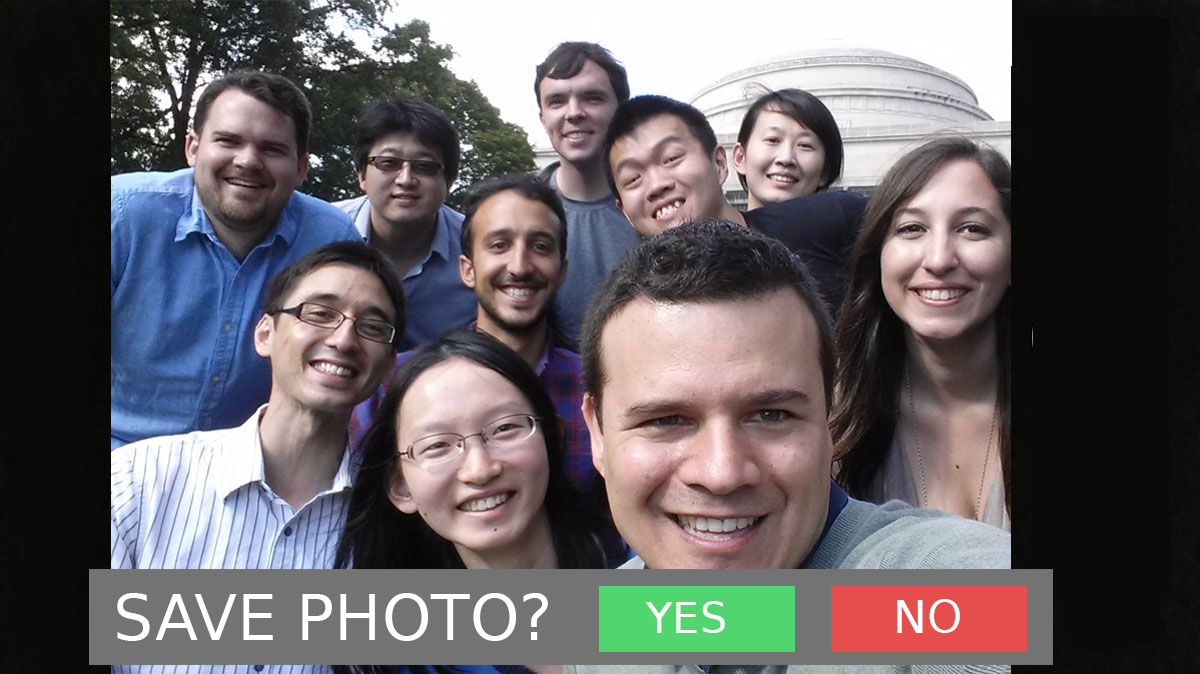
\includegraphics[width=0.75\textwidth]{conceptualmodel2}
    \caption{Mockup demonstrating the approval dialogue}
    \label{fig:conceptualmodel2}
\end{figure}

If the user chooses to accept the photo, then it will be saved to the user's storage and they will return to the camera screen. If the user chooses to discard the photo, then it will be delete and they will return to the camera.




\chapter{Architectural Diagram}

We plan to utilize a data flow architecture to complete this project as shown in Figure 6.1.

\begin{figure}[!h]
    \centering
    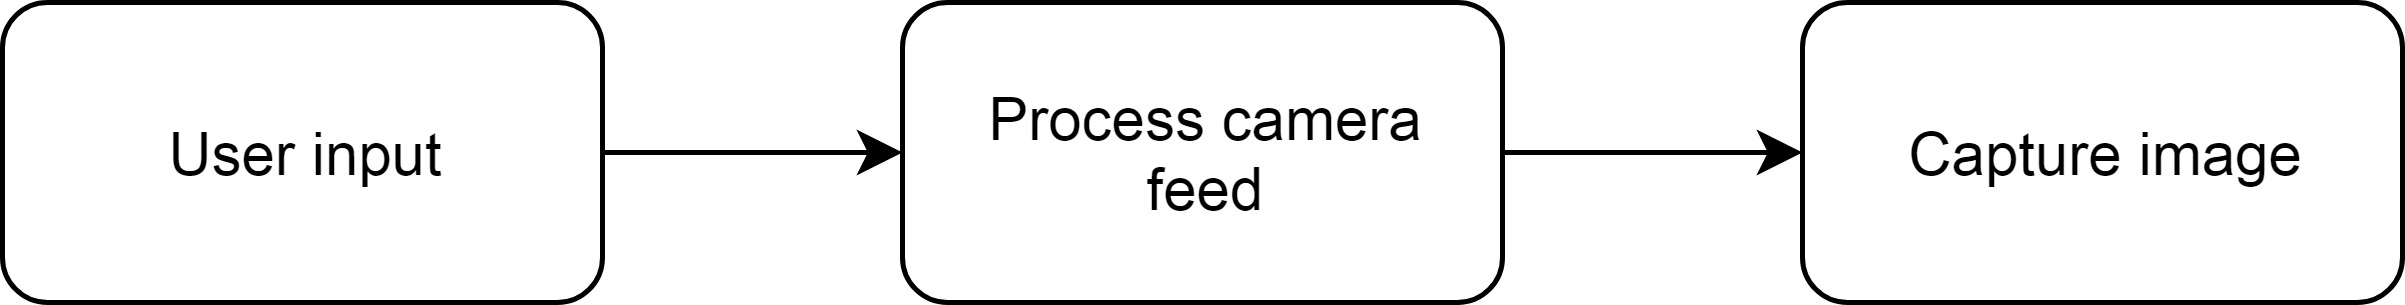
\includegraphics[width=0.75\textwidth]{architecturediagram}
    \caption{Figure 5.1: Data Flow Architecture}
    \label{fig:architecturediagram}
\end{figure}

Users will provide input with their phone's touchscreen, which triggers the device to begin analyzing the camera feed. Once the system determines the input is acceptable, it captures the image.



\backmatter
\end{document}
